\chapter{Data transmission}


One of the most important part of our dissertation project is the data transmission between client and server. In our case the transmission object is image data. The memory size of image depends on quality of the image and its size. 

\section{Processing frames of images}
We tested and developed the project using the web camera of the simple laptop. The laptop’s camera has 2mpx which means the size of the image will be approximately 1MB. actually when we talk about image we consider that we are taking the images from the video stream. The video stream is a collection of frames put together to give one video stream. In average video stream has approximately 25frames per second which means 25 images per second captured by the web camera. after the stage where we got the rectangle image, which shows actually the region of interest, we transmit this image to the server where everyone who are interested can attend the class virtually.

During the research was made 3 steps for image data transmission:
\begin{enumerate}
    \item Send image
    \item Send differences between images
    \item Send segments of differences
\end{enumerate}

Let’s consider that the size of the image as 600x800px which means it has 600 rows and 800 columns. Each pixel stores information about it’s RGB (red, green, blue). a color in the RGB color model is described by indicating how much of each of the red, green, and blue is included. The color is expressed as an RGB triplet (r,g,b), each component of which can vary from zero to a defined maximum value. If all the components are at zero the result is black; if all are at maximum, the result is the brightest representable white.

These ranges may be quantified in several different ways:
\begin{itemize}
    \item From 0 to 1, with any fractional value in between. This representation is used in theoretical analyses, and in systems that use floating point representations.
    \item Each color component value can also be written as a percentage, from 0% to 100%.
    \item In computers, the component values are often stored as integer numbers in the range 0 to 255, the range that a single 8-bit byte can offer. These are often represented as either decimal or hexadecimal numbers.
\end{itemize}


For sending such image we spend the exact amount of the image. If its weight is 1,5MB it send it as a file to server were it will be represented. When working with digital image files, it is essential to know the differences between each one, so you know when to use them. The main difference between files formats is how they are used when designing for the web and the outcome they produce. One produces highly optimized simple graphics, another is used for most images, and the third option is used for complex graphics, gradients and transparency. There can be used several types of images

The color of each pixel of the digital image is described by a few numbers (depending on the color system used). The number of bits to be allowed to represent the color information for each pixel, called the color depth (color depth) or bit color depth (bit depth). Sometimes the color depth is the maximum number of colors that can be represented.

However the work was done on colorful image each pixel has own color depth. Color depth defines how many colors can be used for displaying one pixel. For example, if the color depth is 1 bit, then the pixel can represent only one of two colors - black or white. If the color depth is 8 bits, the number of possible colors is 28 = 256. When the color depth to 24-bit color number over 16 million, which is actually superior to the human eye's ability to resolve color. This is called True Color (true color). Due to the fact that the 24 bit representation is inconvenient in terms of image processing. Typically true color mode uses 32 bits. In the case of a 32-bit representations for color information the lower byte tries still describe the color point and higher bytes or controls additional parameters (for example, alpha channel, with information about the mutual exclusion, objects in three-dimensional or image depth) or not in use. It is clear that this representation is increasing the size of the image, but significantly increases the processing speed of its CPU and GPU computer.

also the image has color quantization. Quantization colors is used to obtain a small number of characteristic colors in the image. Quantization problem in this case can be defined as a predetermined number of selection of the "best" of colors available in a full-color image, and replacing all other colors in the image suitable substitutes from this list. Previously, color quantization process was necessary because the computer video system could only work with a limited color palette (usually 256 colors). Now it is used to reduce the size of the image file, create special effects, sharpening borders, etc.

The simplest approach here is to choose a set of colors to the palette with a uniform distribution of each of the color components. It provides a wide range of colors, but it ignores the fact that most of the images do not have a uniform color distribution.

Currently there are several methods of quantization of color. One of the most effective is the method of color quantization median section. This color space is considered as a three-dimensional cube. Each axis of the cube corresponds to one of the three primary colors: red, green or blue. Each of the three parties is broken into 255 equal parts, the axes are numbered from 0 to 255, wherein the larger value corresponds to a higher color intensity. Method median section 256 divides the cube parallelepiped, each of which contains about the same number of pixels. In this partition of the central point of each parallelepiped is the best choice for the color palette. In the area of the cube, which is densely filled with dots is greater parallelepiped, respectively, into a palette gets more colors. and where fewer points will be taken fewer colors. However, none of the color will not be dropped completely, and preference will be given to those colors, which are more common.

The pixel subtraction operator takes two images as input and produces as output a third image whose pixel values are simply those of the first image minus the corresponding pixel values from the second image. It is also often possible to just use a single image as input and subtract a constant value from all the pixels. Some versions of the operator will just output the absolute difference between pixel values, rather than the straightforward signed output. \cite{Pilet}

after the computation and comparing the last image with current image we will get the matrix Q. On matrix we made some computations after what we get only the pixels which are changed. and send them to the server.

and the last optimization step is to send the differences by lines. It is fact that all the drawn images on the board and any other figures can be represented by the collection straight lines. Using the greedy algorithm we find all the lines and send them to the server. This operation will decrease the sending information till 8 times.


\section{Image compression}
Image compression algorithms are divided into two broad classes: lossless and lossy. In the first case during compression image information is stored in its entirety, while the second - partially lost. The first group of methods of compression ensures the recovery of the original image without any loss or distortion. To store the images for further processing formats should be used, such use is compression methods. However, if the image is intended for visual perception, it is not always necessary. In some cases, the original signal already contains such distortion and noise that small loss in coding information (in favor of a high degree of compression) does not spoil the quality of the overall image.

One of the major problems of computer graphics is that so far not found an adequate and unambiguous criterion for assessing the loss of image quality. For images of the observed visually, it is a major source indistinguishability eye and compressed image. Let’s consider some of the methods used image compression.

Group compression. One of the simplest methods of image compression algorithm is RLE (Run Length Encoding - encoding variable-length string). The basic idea of this method is to search for the same pixels in one line. Found a chain of identical elements are replaced by a pair of (repeat count, value) that in some cases significantly reduces data redundancy.

The algorithm is primarily designed for images with large areas of repeating color (business graphics, diagrams, drawings, etc.). The disadvantage of this approach is that in certain situations, it may instead decrease increases the size of the file (e.g., in some cases, while maintaining color photographs).

There are many schemes compression group, one of which can be illustrated as follows:
\begin{itemize}
\item The input data stream: 17 8 54 0 0 0 97 5 16 0 45 23 0 0 0 0 0 3 67 0 0 8
\item The data stream after encoding: 17 8 54 0 3 97 5 16 0 1 45 23 0 5 0 3 67 8
\end{itemize}

Most often used for encoding scheme called PackBits. By analogy with storing negative numbers, each 7-bit source data are replaced by the result to 8 bits. additional ninth bit is interpreted as the compression flag. For example:
Input: 1,2,3,4,2,2,2,2,4

Data after coding: 1,2,3,4,2, & 3.4.

Principle: The sequence is repeated color values are replaced with its value and the number of repetitions. 

Formats: BMP, TIFF, GIF. 

Ratio: 2

Huffman method.This method is named after its developer (1950). The algorithm is based on the assumption that some of the values of the signal are more common than others. If you analyze the histogram of the image, you can see this. This fact can be used for image compression. Used to store the intensity values that are more common, fewer bits than the value itself. The main problem is to separate one from the other value. after all, the different values assigned to a different number of bits. Huffman compression method can be illustrated as follows in Table \ref{tab:huffman}

\begin{longtable}[t]{|p{0.35\textwidth}|p{0.30\textwidth}|p{0.25\textwidth}|}
\caption{Huffman compression}\label{tab:huffman} \\
	\hline
	\textbf{Value} & \textbf{Frequency} & \textbf{Huffman code} \\
	\hline
	\endhead
	a
	& .154
	& 1\\ [2ex]
	\hline 
    B
    & .072
	& 01 \\ [2ex]
	\hline
    C
	& .072
	& 0010\\ [2ex]
	\hline
    D
	& .063
	& 0011\\ [2ex]
	\hline
    E
	& .059
	& 0001\\ [2ex]
	\hline
    F
	& .015
	& 000010\\ [2ex]
	\hline
    G
	& .011
	& 000011\\ [2ex]
	\hline
\end{longtable}

The input data stream: CEGaDFBEa

The data stream after encoding: 0010 0001 000011 1 0011 000010 01 0001 

Grouping byte: (0010 0001) (1 000 011 0) (011 00001) (01 00 0 1 0 1)
The resulting codes are unique in the sense that they can be recorded into the data stream without separators and markers. By the number of zeros before and after 1 recovery program can uniquely determine the value of the item.

This method is sometimes used in a complicated shape when not one encoded value, and the sequence of values. another modification of the method - subject group codes Huffman compression. Formats: TIFF, GIF. aspect Ratio: 3
Method LZW. This method is named in honor of its developer (Lempel, Ziv, Welch). This is a universal method suitable for encoding any signals. Similar to the method of Huffman coding only for elements used codes equal length and codes used for the common sequence elements.

Tabulate all the colors available to compress images. Thus, instead of the pixel color index can be used from the table. The most common colors in the image are less than the index, while rare colors are placed at the end of the table. The color table (palette) are deployed between the header and the actual image. For example, you can see it in Table \ref{tab:lzw}

\begin{longtable}[t]{|p{0.40\textwidth}|p{0.40\textwidth}|}
\caption{LZW compression}\label{tab:lzw} \\
	\hline
	\textbf{Index} & \textbf{Value} \\
	\hline
	\endhead
	0000 & 0\\ [2ex]
	\hline
	0001 & 1\\ [2ex]
	\hline
	0254 & 254\\ [2ex]
	\hline
	0255 & 255\\ [2ex]
	\hline
	0256 & 145 201 4\\ [2ex]
	\hline
	0257 & 243 245\\ [2ex]
	\hline
	4095 & xxx xxx xxx\\ [2ex]
	\hline
\end{longtable}

The input data stream: 123 145 201 4 119 89 243 245 59 11 206 145 201 4 243 245

The data stream after encoding: 123 256 119 89 257 59 11 206 256 257

Developers have offered not only a way to store data, but also well-documented algorithms for compression and decompression of the signal. The method has been patented, standardized and is now used to compress any information. Formats: TIFF, GIF. aspect Ratio: 5

Method LZW, as RLE, better effect on images containing homogeneous, free from noise portions colors. Thus it acts much better than RLE, compressive arbitrary image data, the encoding process is slower and decompression.

Method JPEG. among the methods of lossy compression should be allocated a family JPEG, developed by the Organization Joint Photographers Experts Group. The method is based on the frequency representation of the image and the following assumptions. If the signal applied to the integral transformation (Fourier for example), the result is a frequency representation of the underlying data are the low frequencies. Treble describe the noise and irrelevant details. Removal of 50\% high-frequency information will entail removal of 5\% of the useful information contained in the image.


JPEG-compression begins with splitting the image into square area of 8 x 8 pixels (64 pixels - 64 bytes). These areas are treated independently. after conversion in each group is from 2 to 20 bytes. When restoring the signal to be performed approximation and restored the original region 8 by 8 pixels. You can see in Figure \ref{fig:jpeg_compression} a jpeg compression in process.

For a compressed representation of the signal can be used a variety of conversion. The most appropriate (qualitative) result gives the conversion Karhunen-Loeve, but it is difficult and time consuming to implement. a Fourier transform, but does not give the desired result in the reduction. Proved most suitable DCT (Discrete Cosine Transform, DCT). When using DCT not need to work with complex numbers (source signal and its spectrum is real).

The transformation of the sample 8 to obtain a sample spectrum 8 8 by 8. This low frequency contained in the upper left corner of the spectrum, and high in the bottom right. High frequencies can be reset or store. If present in the range of the following sequence (Figure xy), then it can be encoded using the compression group. at the last stage of compression used Huffman encoding method for more efficient compression of the resulting data. Principle: Use lossy compression technique. It stores no information about the color of the pixel, and the coefficients of the expansion in some basis. Formats: JPEG 
aspect ratio: depending on the quality of 10 to 1000.


Positives JPEG algorithm is that the user can control the ratio size / quality, the compression ratio setting. Output color image can be color depth of 24 bits per pixel. With the JPEG algorithm achieved high compression ratio with high visual image quality. The negative side of the algorithm is that with an increase in quality, the image is divided into individual square area (size 8x8). This is due to the fact that there are large losses in the low frequencies in the quantization, and restore the original data becomes impossible. additionally, you may be shown the so-called Gibbs effect - halos on the borders of abrupt color transitions. Furthermore, since it a lossy compression algorithm, the processed image with its use is not practical for analysis and further processing.


\begin{figure}[h]
    \centering
    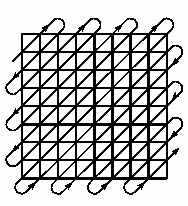
\includegraphics[width=0.5\textwidth]{Figures/jpeg_compression}
    \caption{JPEG compression}
    \label{fig:jpeg_compression}
\end{figure}


\section{Video compression}
Digital image of the storage takes large amounts of memory. Since bitmap 1024 to 1024 pixels with a color depth of 24 bits is a 3 MB. It is understood that the storage and transmission of images in this way is a very time consuming task. Therefore, the problem of representing images in a compact form (data compression) is very important. This should be developed algorithms for encoding and decoding (recovery) images.

There are days, video quality requirements are constantly growing. The width of the channel and container carriers could not keep up with this growth, if not improved video compression algorithm.

Next will talk specifically about some of the basic concepts of video compression. Some are somewhat outdated or described too simple, but it gives the idea of how everything works.

almost everyone knows that any video - this set of static images that will replace each other in time. Then it ordered set we call the video stream. They are different, so are extremely useful to a small classification:

\begin{itemize}
\item Pixel format. a pixel does not give us any information except for his color. However, the perception of color strongly subjective and have been great efforts to create systems tsvetopredstavleniya and color, that would be acceptable to most people. So the color that we see in the real world is hard enough for the range of frequencies of light that transmit it digitally is extremely difficult, and even more difficult to display. However, it was noted that all three points in the spectrum can be accurately displayed colors closer to this metric in color perception ordinary man. These three points of red, green and blue. That is a linear combination, we can cover most of the visible spectrum of colors. Therefore, the easiest way to represent pixel: RGB24, where components for Red, Green and Blue is given exactly 8 bits of information. and so we can pass the 256 gradations of each color, and all sorts of shades 16,777,216. But in practice, the storage tsvetopredstavlenie is almost never used, not only because we are spending as much as 3 bytes per pixel, but also for other reasons, but more on that later (about YV12).
\item Frame size. We have taken all the pixels and coded video and have received a huge amount of data, but it is inconvenient to use. at first, everything is very simple, the frame is characterized by: width, height, and size of the visible part of the format (more on this later). There certainly seem familiar to many figures: 640x480, 720x480, 720x576, 1280x720, 1920x1080. Why is that? Yes, because they appear in different standards, such as 720x576 resolution has most European DVD. No, of course you can make a video size of 417x503, but I do not think that this is something good.
\item aspect ratio. Even knowing the size of the frame, we can not imagine an array of pixels in a more convenient form, without information on how to "package" the frame. In the simplest case, nothing tricky: take a row of pixels in a row and write bits of each coded pixel and so line by line. That is, write down as many rows as we have the height of many pixels as the width and we have everything in order. This is called progressive scan (Progressive). But maybe you're trying to watch TV on your computer without proper settings and saw "comb effect" is when the same object is in different positions with respect to the odd and even lines. It can be a very long time to argue about the appropriateness of interlaced (Interlaced) scan, but the fact that it has remained as a relic of the past by traditional television (someone interested in reading about the device CRT). Pro action (deinterlacing) this unpleasant effect is now not speak. Hence come the magical designations: 576i, 720p, 1080i, 1080p, which indicates the number of rows (the height of the frame) and the type of scan.
\item Frame rate. Some of the standard values: 23.976, 24, 25 and 29.97 fps. For example, 25 f / s used in European television, 29.97 in the US and at 24 f / s on a film shoot. But where did the "strange" 23.976 and 29.97? I will tell you a secret: 23.976 = 24 / 1.001 and 29.97 = 30 / 1.001, ie, in the US television standard NTSC laid divider 1.001. accordingly, when displaying movies happen very slight slowdown that will not be noticeable to the viewer, but if it is a music concert, the display speed is so critical, it is better to occasionally skip frames and again the audience will not notice anything. although I'm a little cheated by the american television never shows "24" frames per second, and shows "30" interlaced frames (and of 59.94 fields per second, which corresponds to the frequency of their power), but they are obtained "by descent" (3: 2 pulldown). The method consists in the fact that we have two full frame and half-frame 5, and the information we have from the first frame filled first half frame 3, and the second the remaining 2. That is, the half-frame sequence is as follows: [1 top, 1 bottom], [1 top, 2 bottom], [2 top, 3 bottom], [3 top, 3 bottom], [4 top, 4 bottom], etc. Where top - upper row (field, fields), a lower bottom, i.e., odd and even from the top, respectively. Thus, the film is quite watchable picture on the TV, but dynamic scenes visible twitching. The frame rate can be variable, but this involves a lot of problems, so consider this case will not.
\item Global characteristics. all the above applications related to local properties, that is, those which are reflected during playback. But the duration time of the video stream, the data capacity, the presence of additional information, and the like, depending For example: the video stream can contain a single stream corresponding left eye and the other stream is some way to store information about the differences between the flow of the right eye from the left. So it is possible to transmit a stereo video or popularly known "3D".
\end{itemize}

Why do you need to compress the video? If we transfer uncompressed video, then anything serious, we had neither the channels of communication or storage space. Suppose we have a HD stream with characteristics: 1920x1080p, 24 f / s, RGB24 and calculate the "cost" of such a flow.

1920 * 1080 * 24 * 24 = 1139 Mbit / s, and if we want to write the 90 minute film, it would take 90 * 60 * 1139 = 750 GB! Cool? This is despite the fact that video film amazing quality with the same 1920x1080p on BluRay will hold 20 GB, that is a difference of almost 40 times!

Obviously, the video compression required, especially given that it is possible to reduce the size to 40 or more times, leaving the audience in raptures.
	
On what the memory of video can be saved:
\begin{itemize}
\item as can be seen, the transformation of linear and non-degenerate. Therefore, we can easily get back to the values of R, G and B. assume for storing Y, U and V, we select 8 bits, then it was 24 bits per pixel, and so it remained. No cost savings. But the human eye is sensitive to brightness, but the color of it is not very pretentious. and almost all color image change each other less frequently. If we divided the image into layers Y, U and V, and luminance layer remain unchanged, and the layers U and V to halve the height and twice the width and order four times. If previously spent on each pixel 24-bit, now spend 8 * 4 + 8 + 8 = 48 bits per pixel 4, that is, roughly speaking, 12 bits per pixel (which is why this is called the encoding format YV12). Due to the decimation of the color we squeezed stream twice without any losses. For example, JPEG always performs this transformation, but compared with other possible artefacts thinning colors carries no harm.

\item The redundancy of the image. There will not dwell too much, as there are no differences from the image compression algorithms. The same JPEG compresses the image by its local redundancy method of discrete cosine transform (DCT) and quantization, as once again can be found on Wikipedia. Outline only what built-in codec compression algorithm of still images must compress well even remotely resembling a real image will soon learn why.

\item Frame difference. Surely, anyone watching any video, notice that the images do not change dramatically, and the adjacent frames are similar enough. Of course, there are swings, but they usually occur when changing scenes. and then there is a problem: the computer has to represent all the variety that can be converted images? Help comes motion compensation algorithm. about it I write an article on Wikipedia. To produce copy-paste, confine highlights. The image is divided into blocks in the vicinity of each block is searched similar to another frame (motion estimation), it turns the field motion vectors. and even when compensation (motion compensation) accounted for the motion vector and creates the overall image is similar to the original frame. Given the volume of information in image compression we can keep the motion vector is almost free. We do this and then squeezed compensated frame difference image compression algorithm of static images. and as the second picture frank medley, the image compression algorithm should correctly work with such things. Due to a large redundancy of such images are compressed very strongly. But if the codec compresses them too much, and there is a block effect. Older algorithms can not account for changes in brightness of objects and that is why you can see on TV blockiness President outbreaks cameras.

\item Organization of successive frames. The first codec must be sensitive to scene change. Define it simply because the motion compensation is fulfilled in this case, the ugly. Still the beginning of a new scene is logical to retain "as is", since it neither had previously found not like. These frames are called reference (I-frame). and then go frames to which the motion compensation, ie, they depend on the reference frame and each other. This may be P-frame or B-frame. The former can only rely on the previous frames, and may last on the left and right neighbor. I-frame and all its dependent manner GOP (group of pictures). From the use of bi-frames should be as advantages: fast navigation (because the previous bi-frames do not need to decode) and the fact that they have the smallest size among all the frames of a movie, well, a little lower quality (but rapid alternation with more quality training It makes it unobtrusive to the viewer).

\item Redundancy output. Even after all the procedures of contracting the flow coefficient is redundancy. Further, various methods can be applied lossless. The codec H.264, for example, there are two options CaBaC and CaVLC, realizing arithmetic compression with strong probabilistic model and implement Huffman with a simple model. For unknown reasons, apple prefers the latter option, although good decoders difference in speed is negligible.


\end{itemize}



Let’s see the sending data in images. Lets consider that we have the image which is represented in matrix in Figure \ref{fig:example_matrix} and lets assume that after some time it was changed and became as in Figure \ref{fig:last_image_matrix}.

\begin{figure}[h]
    \centering
    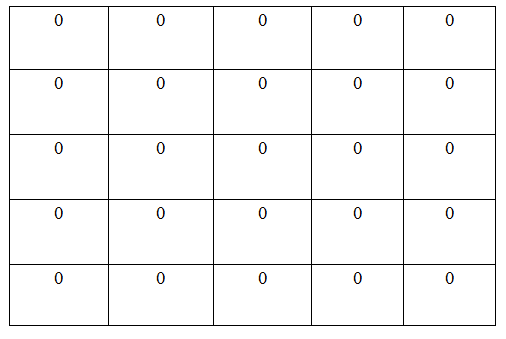
\includegraphics[width=0.5\textwidth, height=0.35\textwidth]{Figures/example_matrix}
    \caption{Initial state of image matrix}
    \label{fig:example_matrix}
\end{figure}

\begin{figure}[h]
    \centering
    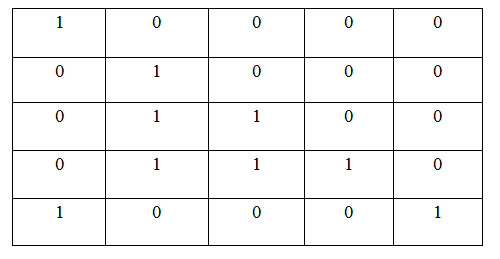
\includegraphics[width=0.5\textwidth, height=0.35\textwidth]{Figures/last_image_matrix}
    \caption{Final state of image matrix}
    \label{fig:last_image_matrix}
\end{figure}


By using the first approach we need to send whole matrix to the server. The memory complexity will be 5x5. By using the second approach we will need to send to the server the only differences seen in Figure \ref{fig:result_matrix}:

\begin{figure}[h]
    \centering
    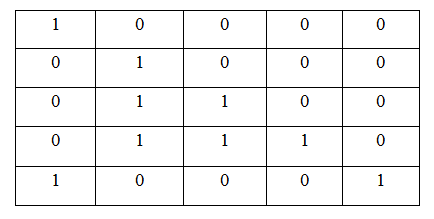
\includegraphics[width=0.5\textwidth, height=0.35\textwidth]{Figures/result_matrix}
    \caption{Resulting matrix}
    \label{fig:result_matrix}
\end{figure}

In our example there are 9 pixels which are changed. In this approach we need to send only this seven pixels. It’s memory complexity is 7(quantity of changed pixels). By using the last approach we will send to the server only the lines. In this method we will used greedy algorithm and try to represent all the pixel as a collection of lines. Lets consider that the beginning coordinate of i-th line will be named as i-b and end of line will named as i-e in Figure \ref{fig:segmentation_result}:

\begin{figure}[h!]
    \centering
    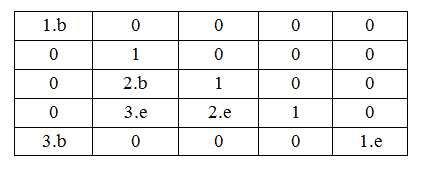
\includegraphics[width=0.5\textwidth, height=0.35\textwidth]{Figures/segmentation_result}
    \caption{Segmentation of matrix}
    \label{fig:segmentation_result}
\end{figure}


In this situation it is enough to send only the 3 lines to server to represent this image. For examples like 5x5 the actually will not be obvious in comparing with 100x100 or 1000x1000 images. The greedy algorithm will be described in technical part of this paper.
